\documentclass[journal,12pt,twocolumn]{IEEEtran}

\usepackage{setspace}
\usepackage{gensymb}

\singlespacing 



\usepackage[cmex10]{amsmath}

\usepackage{amsthm}

\usepackage{mathrsfs}
\usepackage{txfonts}
\usepackage{stfloats}
\usepackage{bm}
\usepackage{cite}
\usepackage{cases}
\usepackage{subfig}

\usepackage{longtable}
\usepackage{multirow}

\usepackage{enumitem}
\usepackage{mathtools}
\usepackage{steinmetz}
\usepackage{tikz}
\usepackage{circuitikz}
\usepackage{verbatim}
\usepackage{tfrupee}
\usepackage[breaklinks=true]{hyperref}
\usepackage{graphicx}
\usepackage{tkz-euclide}
\usepackage{float}

\usetikzlibrary{calc,math}
\usepackage{listings}
    \usepackage{color} %%
    \usepackage{array} %%
    \usepackage{longtable} %%
    \usepackage{calc} %%
    \usepackage{multirow} %%
    \usepackage{hhline} %%
    \usepackage{ifthen} %%
    \usepackage{lscape}     
\usepackage{multicol}
\usepackage{chngcntr}
\newcommand{\norm}[1]{\left\lVert#1\right\rVert}

\DeclareMathOperator*{\Res}{Res}

\renewcommand\thesection{\arabic{section}}
\renewcommand\thesubsection{\thesection.\arabic{subsection}}
\renewcommand\thesubsubsection{\thesubsection.\arabic{subsubsection}}

\renewcommand\thesectiondis{\arabic{section}}
\renewcommand\thesubsectiondis{\thesectiondis.\arabic{subsection}}
\renewcommand\thesubsubsectiondis{\thesubsectiondis.\arabic{subsubsection}}


\hyphenation{op-tical net-works semi-conduc-tor}
\def\inputGnumericTable{} %%

\lstset{
%language=C,
frame=single, 
breaklines=true,
columns=fullflexible
}
\begin{document}


\newtheorem{theorem}{Theorem}[section]
\newtheorem{problem}{Problem}
\newtheorem{proposition}{Proposition}[section]
\newtheorem{lemma}{Lemma}[section]
\newtheorem{corollary}[theorem]{Corollary}
\newtheorem{example}{Example}[section]
\newtheorem{definition}[problem]{Definition}

\newcommand{\BEQA}{\begin{eqnarray}}
\newcommand{\EEQA}{\end{eqnarray}}
\newcommand{\define}{\stackrel{\triangle}{=}}
\newcommand\hlight[1]{\tikz[overlay, remember picture,baseline=-\the\dimexpr\fontdimen22\textfont2\relax]\node[rectangle,fill=blue!50,rounded corners,fill opacity = 0.2,draw,thick,text opacity =1] {$#1$};}
\bibliographystyle{IEEEtran}
\providecommand{\mbf}{\mathbf}
\providecommand{\pr}[1]{\ensuremath{\Pr\left(#1\right)}}
\providecommand{\qfunc}[1]{\ensuremath{Q\left(#1\right)}}
\providecommand{\sbrak}[1]{\ensuremath{{}\left[#1\right]}}
\providecommand{\lsbrak}[1]{\ensuremath{{}\left[#1\right.}}
\providecommand{\rsbrak}[1]{\ensuremath{{}\left.#1\right]}}
\providecommand{\brak}[1]{\ensuremath{\left(#1\right)}}
\providecommand{\lbrak}[1]{\ensuremath{\left(#1\right.}}
\providecommand{\rbrak}[1]{\ensuremath{\left.#1\right)}}
\providecommand{\cbrak}[1]{\ensuremath{\left\{#1\right\}}}
\providecommand{\lcbrak}[1]{\ensuremath{\left\{#1\right.}}
\providecommand{\rcbrak}[1]{\ensuremath{\left.#1\right\}}}
\theoremstyle{remark}
\newtheorem{rem}{Remark}
\newcommand{\sgn}{\mathop{\mathrm{sgn}}}
%\providecommand{\abs}[1]{\left\vert#1\right\vert}
\providecommand{\res}[1]{\Res\displaylimits_{#1}} 
\providecommand{\norm}[1]{$\left\lVert#1\right\rVert$}
%\providecommand{\norm}[1]{\lVert#1\rVert}
\providecommand{\mtx}[1]{\mathbf{#1}}
%\providecommand{\mean}[1]{E\left[ #1 \right]}
\providecommand{\fourier}{\overset{\mathcal{F}}{ \rightleftharpoons}}
%\providecommand{\hilbert}{\overset{\mathcal{H}}{ \rightleftharpoons}}
\providecommand{\system}{\overset{\mathcal{H}}{ \longleftrightarrow}}
 %\newcommand{\solution}[2]{\textbf{Solution:}{#1}}
\newcommand{\solution}{\noindent \textbf{Solution: }}
\newcommand{\cosec}{\,\text{cosec}\,}
\providecommand{\dec}[2]{\ensuremath{\overset{#1}{\underset{#2}{\gtrless}}}}
\newcommand{\myvec}[1]{\ensuremath{\begin{pmatrix}#1\end{pmatrix}}}
\newcommand{\mydet}[1]{\ensuremath{\begin{vmatrix}#1\end{vmatrix}}}
\numberwithin{equation}{subsection}
\makeatletter
\@addtoreset{figure}{problem}
\makeatother
\let\StandardTheFigure\thefigure
\let\vec\mathbf
\renewcommand{\thefigure}{\theproblem}
\def\putbox#1#2#3{\makebox[0in][l]{\makebox[#1][l]{}\raisebox{\baselineskip}[0in][0in]{\raisebox{#2}[0in][0in]{#3}}}}
     \def\rightbox#1{\makebox[0in][r]{#1}}
     \def\centbox#1{\makebox[0in]{#1}}
     \def\topbox#1{\raisebox{-\baselineskip}[0in][0in]{#1}}
     \def\midbox#1{\raisebox{-0.5\baselineskip}[0in][0in]{#1}}
\vspace{3cm}
\title{Assignment-07}
\author{Suyog Tangade \\ MD/2020/710}
\maketitle
\newpage
\bigskip
\renewcommand{\thefigure}{\theenumi}
\renewcommand{\thetable}{\theenumi}
Download latex-tikz codes from
\begin{lstlisting}
https://github.com/suyogtangade/Assignment7.git
\end{lstlisting}
%
Download python codes from
\begin{lstlisting}
https://github.com/suyogtangade/Assignment7.git
\end{lstlisting}
%
Question taken from
\begin{lstlisting}
  https://github.com/gadepall/ncert/blob/main/linalg/optimization/gvv_ncert_opt.pdf question 2.14
\end{lstlisting}
\section{Question No 2.14}
 There are two types of fertilisers $F_{1}$ and $F_{2}$.$F_{1}$ consists of $10\%$ nitrogen and $6\%$
phosphoric acid and $F_{2}$ consists of $5\%$ nitrogen and $10\%$ phosphoric acid. After
testing the soil conditions, a farmer finds that she needs atleast 14 kg of nitrogen
and 14 kg of phosphoric acid for her crop. If $F_{1}$ costs Rs 6/kg and $F_{2}$ costs
Rs 5/kg, determine how much of each type of fertiliser should be used so that
nutrient requirements are met at a minimum cost. What is the minimum cost?\\
\section{Solution}
\begin{table}[!ht]
\centering
\resizebox{\columnwidth}{!}{\begin{tabular}{|c|c|c|c|c|} 
\hline
Fertiliser  & Nitrogen  & Phosphoric acid  & Quantity  & Cost \\
\hline
F1 & 10 Percentage & 6 Percentage & X Kg  & Rs 6 \\
\hline
F2 & 5 Percentage & 10 Percentage  &  Y Kg  & Rs 5 
\\
\hline
Total & 14 Kg & 14Kg &  &
\\
\hline
\end{tabular}}
\label{opt/16/tab:table1}
\end{table}
\item Lets consider fertiliser F1 requirement is x kg \\
fertiliser F2 requirement is y kg 
\begin{align}
    x \geq 0 \\
    y \geq 0 
\end{align}
According to the question,
\begin{align}
    10x+5y &\leq 14 \\
\end{align}
     and,
\begin{align}
    6x+10y &\leq 14 \\
 \implies 3x+5y &\leq 7
\end{align}
$\therefore$ Our problem is
\begin{align}
        \max_{\vec{x}} Z &= \myvec{6 & 5}\vec{x}\\
        s.t. \quad 
        \myvec{10 & 5 \\ 3 & 5 }\vec{x} &\preceq \myvec{14\\7} 
\end{align}
Lagrangian function is given by
\begin{equation}
\begin{aligned}
    &L(\vec{x},\boldsymbol{\lambda}) \\ &= \myvec{6 & 5}\vec{x}+\lcbrak{\sbrak{\myvec{10 & 5}\vec{x}+14}} \\ &+ \sbrak{\myvec{3 & 5}\vec{x}+7} \\ &+ \sbrak{\myvec{-1 & 0}\vec{x}} +\rcbrak{\sbrak{\myvec{0 & -1}\vec{x}}}\boldsymbol{\lambda}
\end{aligned}
\end{equation}
where,
\begin{align}
    \boldsymbol{\lambda} &= \myvec{\lambda_1 \\ \lambda_2 \\ \lambda_3 \\ \lambda_4 \\ \lambda_5 \\ \lambda_6}
\end{align}
Now,
\begin{align}
    \nabla L(\vec{x},\boldsymbol{\lambda}) &= \myvec{6+ \myvec{10 & 5 & -1 & 0 }\boldsymbol{\lambda}\\ 6+\myvec{3 & 5 & 0 & -1}\boldsymbol{\lambda} \\ \myvec{10 & 5}\vec{x}+14 \\ \myvec{3 & 5}\vec{x}+7 \\ \myvec{-1 & 0}\vec{x} \\ \myvec{0 & -1}\vec{x}}
\end{align}
$\therefore$ Lagrangian matrix is given by
\begin{align}
    \myvec{0 & 0 & 10 & 5 & -1 & 0 \\ 0 & 0 & 3 & 5 & 0 & -1 \\ 10 & 5 & 0 & 0 & 0 & 0  \\ 3 & 5 & 0 & 0 & 0 & 0  \\ -1 & 0 & 0 & 0 & 0 & 0  \\ 0 & -1 & 0 & 0 & 0 & 0 }\myvec{\vec{x} \\ \boldsymbol{\lambda} } &= \myvec{-6 \\ -5 \\ 14 \\ 7 \\ 0 \\0 }
\end{align}
Considering $\lambda_1,\lambda_2$ as only active multiplier,
\begin{align}
    \myvec{0 & 0 & 10 & 5 \\ 0 & 0 & 3 & 5 \\ 10 & 5 & 0 & 0 \\ 3 & 5 & 0 & 0}\myvec{\vec{x}\\ \boldsymbol{\lambda}} &=\myvec{-6 \\ -5 \\ 14 \\ 7}
\end{align}
resulting in,
\begin{align}
    \myvec{\vec{x} \\ \boldsymbol{\lambda}} &= \myvec{0 & 0 & 10 & 5 \\ 0 & 0 & 3 & 5 \\ 10 & 5 & 0 & 0 \\ 3 & 5 & 0 & 0}^{-1}\myvec{-6 \\ -5 \\ 14 \\ 7}
    \\
    \implies   \myvec{\vec{x} \\ \boldsymbol{\lambda}} &= \myvec{0 & 0 & \frac{1}{7} & \frac{-1}{7} \\ 0 & 0 & \frac{-3}{35} & \frac{2}{7} \\ \frac{1}{7} & \frac{-1}{7} & 0 & 0 \\ \frac{-3}{35} & \frac{2}{7} & 0 & 0}\myvec{-6 \\ -5 \\ 14 \\ 7}
    \\
    \implies \myvec{\vec{x} \\ \boldsymbol{\lambda}} &= \myvec{1 \\ \frac{4}{5} \\ \frac{-1}{7} \\ \frac{-32}{35} }
\end{align}
$\because \boldsymbol{\lambda}=\myvec{\frac{-1}{7} \\ \frac{-23}{35}} \succ \vec{0} $ 
\\
$\therefore$ Optimal solution is given by
\begin{align}
    \vec{x} &= \myvec{1\\\frac{4}{5}} \\
    Z &= \myvec{6 & 5}\vec{x} \\
    &= \myvec{6 & 5}\myvec{1 \\\frac{4}{5} } \\
    &= 10
\end{align}
By using cvxpy in python ,
\begin{align}
    \vec{x}=\myvec{1\\0.8}\\
    Z = 10
\end{align}
Hence the cost will be minimum If fertilizer F1 used  \boxed{x=1kg} and fertilizer F2 used  \boxed{y=\frac{4}{5}} \\ Minimum cost   \boxed{Z=10}.  This
is verified in Fig. \ref{fig: Optimization graphical solution}.	
%
\begin{figure}[!ht]
\centering
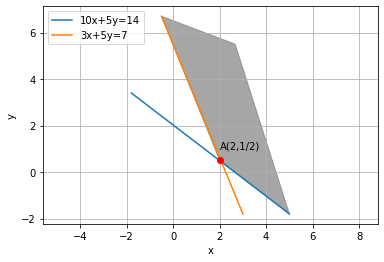
\includegraphics[width=\columnwidth]{Optimization.png}
\caption{graphical solution}
\label{fig: Optimization graphical solution}	
\end{figure}


\end{document}